\clearpage
\appendix

\section{Pseudo code of \workname}\label{Pseudo Code}
The training pseudo code of \workname  is as follows:

% \documentclass[11pt]{article}
% \usepackage{CJK}
% \usepackage[top=2cm, bottom=2cm, left=2cm, right=2cm]{geometry}
% \usepackage{amsmath}
% \usepackage{indentfirst}

% \floatname{algorithm}{算法}
% \renewcommand{\algorithmicrequire}{\textbf{输入:}}
% \renewcommand{\algorithmicensure}{\textbf{输出:}}

% TODO Repaint the pseudo code
\begin{algorithm}
    \caption{DeCLIP}
    \begin{algorithmic}[1] %每行显示行号
        \Require $I$, $\tilde{I}$, $T$, $\tilde{T}$, $image\_encoder$, $text\_encoder$, $Feature\_Queue$
        % \Ensure $Logits$
        \Function {Batch-Updating}{$I$, $\tilde{I}$, $T$, $\tilde{T}$}
            \State \textcolor[RGB]{64,128,128}{$\#$ Get The Features of The Current Batch.}
            % \State $I_f \gets image\_encoder(I)$
            % \State $\tilde{I}_f \gets image\_encoder(\tilde{I})$
            % \State $T_f \gets text\_encoder(T)$
            % \State $\tilde{T}_f \gets text\_encoder(\tilde{T})$
            \State $I_f, \tilde{I}_f \gets image\_encoder(I), image\_encoder(\tilde{I})$
            \State $T_f, \tilde{T}_f \gets text\_encoder(T), text\_encoder(\tilde{T})$
            \State $T_{NN} \gets$ \Call{Nearest-Neighbor}{$Feature\_Queue, T_f$}
            \State
            \State \textcolor[RGB]{64,128,128}{$\#$ Calculate The losses.}
            \State $L_{CLIP} \gets$ \Call{InfoNCE-Loss}{$I_f, T_f$}
            \State $L_{SS} \gets$ \Call{Image-SS-Loss}{$I_f, \tilde{I}_f$} + \Call{Text-SS-Loss}{$T_f$}
            \State $L_{MVS} \gets$ \Call{InfoNCE-Loss}{$I_f, \tilde{T}_f$} + \Call{InfoNCE-Loss}{$\tilde{I}_f, T_f$} + \Call{InfoNCE-Loss}{$\tilde{I}_f, \tilde{T}_f$}
            \State $L_{NNS} \gets$ \Call{InfoNCE-Loss}{$\tilde{I}_f, \tilde{T}_{NN}$}
            \State $L_{\workname} \gets (1 - \alpha - \beta - \gamma)L_{CLIP} + \alpha L_{SS} + \beta L_{MVS} + \gamma L_{NNS}$
            \State
            \State \textcolor[RGB]{64,128,128}{$\#$ Update The Network.}
            % \State \Call{Update-NetWork}{$image\_encoder, L_{\workname}$}
            % \State \Call{Update-NetWork}{$text\_encoder, L_{\workname}$}
            % \State $Feature\_Queue \gets$ \Call{Update-FeatureQueue}{$Feature\_Queue, T_f$}
            \State $image\_encoder \gets$ \Call{Backward-Update}{$image\_encoder, L_{\workname}$}
            \State $text\_encoder \gets$ \Call{Backward-Update}{$text\_encoder, L_{\workname}$}
            \State $Feature\_Queue \gets$ \Call{FIFO-Update}{$Feature\_Queue, T_f$}
        \EndFunction
        \State
        \Function {Image-SS-Loss}{$I_f, \tilde{I}_f$}
            \State $z, \tilde{z} \gets image\_encoder.proj(I_f), image\_encoder.proj(\tilde{I}_f)$
            \State $p, \tilde{p} \gets image\_encoder.pred(z), image\_encoder.pred(\tilde{z})$
            \State $z, \tilde{z} \gets z.detach(), \tilde{z}.detach()$
            \State \textcolor[RGB]{64,128,128}{$\#$ Calculate the Negative Cosine Similarity loss.}
            \State $L_{Image-SS} \gets NCS(p, \tilde{z}) / 2 + NCS(\tilde{p}, z) / 2$  
            \State \Return{$L_{Image-SS}$}
        \EndFunction
        \State
        \Function {Text-SS-Loss}{$T_f$}
            \State \textcolor[RGB]{64,128,128}{$\#$ Get The Masking GT when performing the text-encoder.}
            \State $W_f, W_{gt} \gets T_f.word\_feat, T_f.mask\_id$
            % \textcolor{gray}{$\#$ $W_f$ and $W_{gt}$ represents the features and masked words, respectively.}
            \State $W_{pred} \gets text\_encoder.pred(W_f)$
            \State \textcolor[RGB]{64,128,128}{$\#$ Calculate the Cross-Entropy loss.}
            \State $L_{Text-SS} \gets CE(W_{gt}, W_{pred})$  
            \State \Return{$L_{Text-SS}$}
        \EndFunction
        
    \end{algorithmic}
\end{algorithm}


\section{Data Augmentation}\label{data_aug}

\paragraph{Details of SS} The image SS uses SimSiam~\citep{chen2021exploring} method as the image self-supervision. The prediction module is a 2-layer MLP, in which the hidden dimensions are 512 and output dimensions are 1024, the projection module is a 3-layer MLP, in which the hidden and output dimensions are both 1024. The text SS uses the Masked Language Model~\citep{devlin2018bert} as the pretext task. In detail, we first randomly choose $15\%$ of all tokens in each sequence. Then the token is replaced with (1) the \texttt{[mask]} token $80\%$ of the time (2) a random token $10\%$ of the time (3) the unchanged token $10\%$ of the time.

\paragraph{Image augmentations} The augmentation policy includes: \texttt{RandomResizedCrop} with scale in [0.2,1.0]~\citep{wu2018unsupervised}, \texttt{ColorJitter} containing \{brightness, contrast, saturation, hue\} strength of \{0.4, 0.4, 0.4, 0.1\} with an applying probability of 0.8, \texttt{RandomGrayscale} with an applying probability of 0.2. Blurring augmentation~\citep{chen2020simple} has a Gaussian kernel with std in [0.1, 2.0], and \texttt{RandomHorizontalFlip}.

\paragraph{Text augmentations} We use the EDA~\citep{wei2019eda} method as our text augmentation strategy, which contains three types of text augmentation strategies: synonym replacement, random swap, and random deletion. Each text will randomly select one of these three types for text augmentation.
%EDA has four types of text augmentation: synonym replacement, random insertion, random swap, and random deletion. 



\section{Pre-training datasets \& implementation details}\label{app: pretrain details}

\paragraph{Open-source data.} Conceptual Captions~\citep{sharma2018conceptual} is a 3.3 M image caption open-source data. Due to the failure of the download link, we only download about 3M data(CC3M). 
Conceptual 12M~\citep{sharma2018conceptual} contains approximately 12M of image-text pairs(CC12M), which is larger than the CC3M and covers a more diverse set of visual concepts. Also, due to the failure of the download link, we only download about 11M data. 
YFCC~\citep{thomee2016yfcc100m}, the Yahoo Flickr Creative Commons 100M data, is a dataset for vision language tasks. We download about 86.5M data from the YFCC website and use four filtering rules to filter the \workname YFCC15M dataset to benchmark against CLIP YFCC15M. The four rules are: filtering data with damaged images, filtering data without the caption, filtering data with a caption English word ratio less than 0.8, filtering data with a caption only including one part of speech. 

\paragraph{Web-crawled data.} We use the user tags and machine tags of YFCC15M to form a tag list, and use WordNet~\citep{miller1995wordnet} to find synonyms for each tag in the tag list to form a synonym tag list. The tag list and synonym tag list form a query list. Then we use the query list to crawl images from the Internet, after filtering data with smaller images, filtering data with damaged images, filtering data without the caption, and filtering data with Chinese in the caption, we collect 59M web crawled data.
Tabel \ref{tab:pretrain datasets api} shows the source link of pre-training datasets, and Figure \ref{fig:sample case} shows some cases random sampled from each dataset.

\begin{figure}[h]
	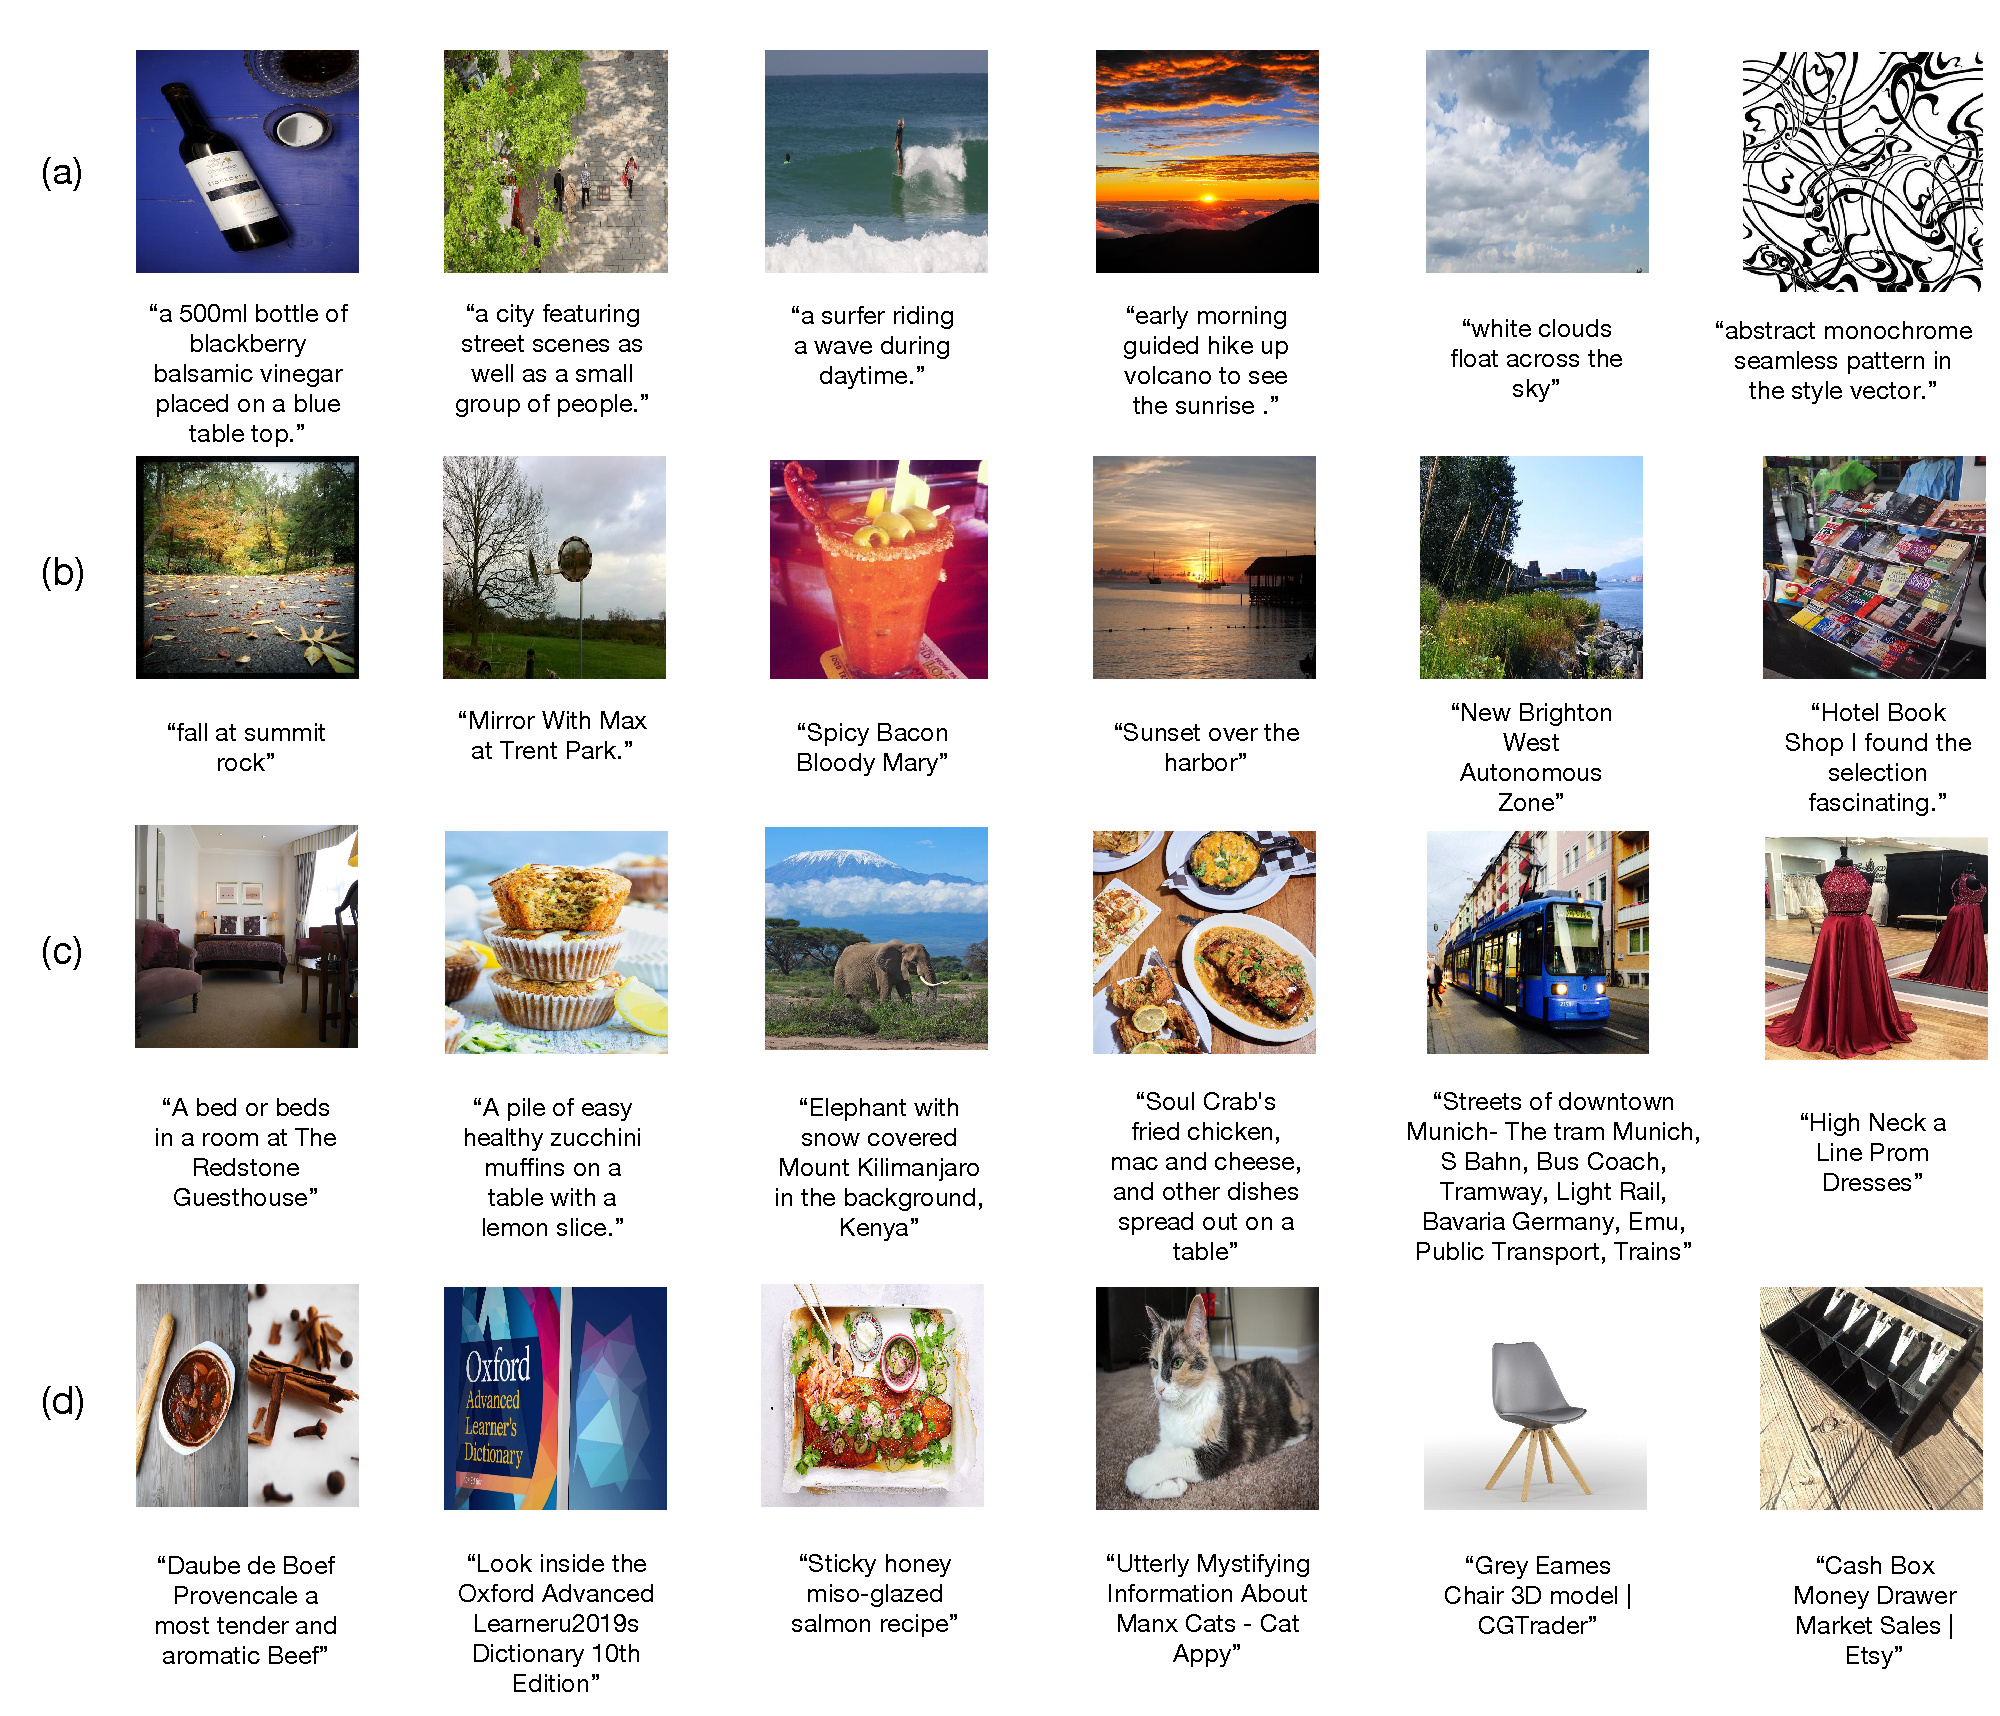
\includegraphics[width=1.0\columnwidth]{DeCLIP/figs/check-pickv5.pdf}
    \vskip -0.2in
	\caption{ Example image-text pairs randomly sampled from the training dataset. (a) Conceptual Captions, (b) YFCC, (c) Conceptual 12M, (d) Web-crawled.}
	\label{fig:sample case}
\end{figure}


\begin{table*}[h]
\caption{\label{tab:pretrain datasets api}The source link of DeCLIP pre-training datasets.}
\label{sample-table}
\begin{center}
\begin{small}
\begin{sc}
\begin{tabular}{lr}
   \toprule  
   %\multicolumn{5}{r}{}  \\
   \textbf{Dataset}      &\textbf{Dataset Api} \\
   \midrule   
   ConceptualCaptions         &https://ai.google.com/research/ConceptualCaptions      \\
   Conceptual12M              &https://github.com/google-research-datasets/conceptual-12m \\
   YFCC                        &http://projects.dfki.uni-kl.de/yfcc100m      \\
   Google                      &https://www.google.com.hk \\ 
   \bottomrule
   
\end{tabular}
\end{sc}
\end{small}
\end{center}
\end{table*}

\paragraph{Implementation details} We train \workname-ResNet50 (abbr. as R50) and \workname-ViT-B/32 (abbr. as V-B32) from scratch for 32 epochs.
For R50, we use the FP16-SGD optimizer with the batch size of 10,240 (128$\times$80). Starting with an 0.01 learning rate (lr), we first linearly increasing the lr to 0.2 (a.k.a warm-up) in one epoch. Then we use cosine anneal lr decay to decrease the lr. The weight decay is set to 0.0001.
% All experiments are using cosine learning rate decay.
For V-B32, we use a hybrid FP16-AdamW-SGD optimizer with bacth size 10,240(128$\times$80). For the ViT image encoder, we use AdamW optimizer with the lr warming up from 1e-4 to 1e-3 in one epoch. The weight decay is set to 0.05. For the text encoder, we use the SGD optimizer with the lr warming up from 1e-3 to 0.02 in one epoch. The weight decay is set to 1e-4.

% ResNet-50 uses the FP16-SGD optimizer and batch size 10,240  for training, with an initial learning rate of 0.01, warmed up linearly to 0.2 in one epoch steps, which weight decay is 0.0001 and momentum is 0.9.
% When training ViT-B/32, we use FP16-AdamW-SGD with batch size 20,480 for stable training. In detail, When training the text encoder, we use the SGD optimizer which learning rate warmed up linearly from 1e-3 to 0.02, the weight decay rate is set as 1e-4 and the momentum is set as 0.9. For the image encoder, we use AdamW optimizer which learning rate warmed up linearly from 1e-4 to 1e-3, and the weight decay rate is set as 0.05.


\paragraph{Pre-training cost} Our R50 and V-B32 took 8/10 days to train on 80 V100 GPUs, respectively. Our largest \workname-RegNetY-64GF took 21 days on 160 V100 GPUs, while the largest CLIP-R50$\times$64 from ~\citep{radford2021learning} spent 18 days on 592 V100 GPUs.

\section{Downstream Datasets \& implementation details}\label{Downstream Datasets}

\paragraph{Downstream data.} We begin with the 12 datasets from the well-studied evaluation suite introduced by ~\citet{kornblith2019better}. 
Within these 12 datasets, Birdsnap can not be downloaded, and PASCAL VOC 2007 classification is replaced by more challenging ImageNet-1K, resulting in our 11 datasets.
They are: Food-101, CIFAR-10, CIFAR-100, SUN397, Stanford Cars, FGVC Aircraft, Describable Textures, Oxford-IIIT Pets, Caltech-101, Oxford Flowers 102. Tab.~\ref{tab:downstream datasets} is the detailed information of these datasets.


\begin{table*}[h]
\caption{\label{tab:downstream datasets} Details of DeCLIP downstream datasets.}
\label{sample-table}
\begin{center}
\begin{small}
\begin{sc}
\begin{tabular}{lcccr}
   \toprule  
   %\multicolumn{5}{r}{}  \\
   \textbf{Dataset}         & \textbf{Classes}  & \textbf{Train Size } &  \textbf{Test Size}  & \textbf{Evaluation Metric } \\
   \midrule   
   CIFAR10         & 10  	  &  50,000	     &     10,000      & accuracy	\\
   CIFAR100        & 100     &  50,000      &     10,000      & accuracy   \\
   Food-101	       & 101     &  75,750      &     25,250      & accuracy   	\\
   OxfordIIIT-Pets & 37      &  3,680       &     3,669       & mean per class \\
   Oxford 102 Flowers  & 102    & 2,040     &     6,149       & mean per class \\
   SUN          & 397     & 19,850       &     19,850      & accuracy \\
   Stanford Cars   & 196     & 8,144        &     8,041       & accuracy \\
   DTD             & 47      & 3,760        &     1,880       & accuracy \\    
   Caltech-101     & 102     & 3,060        &     6,085       & mean per \\
   FGVC Aircraft   & 100     & 6,667        &     3,333       & mean per class \\
   ImageNet1k     & 1000    & 1,281,167    &     50,000      & accuracy \\
  \bottomrule
\end{tabular}
\end{sc}
\end{small}
\end{center}
\end{table*}

\paragraph{Implementation details} We follow CLIP~\citep{radford2021learning} to train a logistic regression classifier using L-BFGS, with maximum 1,000 iterations, and report the corresponding metric for each dataset. We determine the L2 regularization strength $\lambda$ using a hyperparameter sweep on the validation sets over the range between $10^{-6}$ and $10^6$, with 96 logarithmically spaced steps. To save compute required for the sweeps, we perform a parametric binary search that starts with $\lambda$ = [$10^{-6}$, $10^{-4}$, $10^{-2}$, 1, $10^2$, $10^4$, $10^6$] and iteratively halves the interval around the peak until it reaches a resolution of 8 steps per decade. The hyperparameter sweeps are performed on a validation split of each dataset. For the datasets that contains a validation split in addition to from the test split, we use the provided validation set to perform the hyperparameter search, and for the datasets that do not provide a validation split or have not published labels for the test data, we split the training dataset to perform the hyperparameter search and report the performance on the validation data.

% For each dataset, the image features are firstly extracted using the pre-trained image encoder to form a full-batch. The input resolution for train and eval part are both $224\times224$ \checkme{with frozen visual features?}.
% % Both train and eval resolution are $224\times224$ with frozen visual features.
% Secondly, we train a fc-based classifier by the L-BFGS optimizer with 1,000 full-batch iterations.
% Finally, we determine the L2 regularization strength using a hyperparameter $\lambda$ sweep on the validation sets over the range between 1e-6 and 1e6 with 16 logarithmically spaced steps. \checkme{Maybe we can copy this part from CLIP.}





\section{Prompt Engineering}\label{Prompts}

% As shown in ~\cite{radford2021learning}, 
Due to the reason that it's relatively rare in the dataset for the text to be a single word, we use prompts such as  \texttt{"a photo of a \{label\}"} for zero-shot classification. For a fair comparison, we use the same prompts as proposed in ~\cite{radford2021learning} for the ImageNet dataset. As shown in Fig~\ref{fig:prompts}, the prompts reduce the domain gap between the training dataset and testset, and fully consider the different situations for the picture.

\begin{figure}[h]
	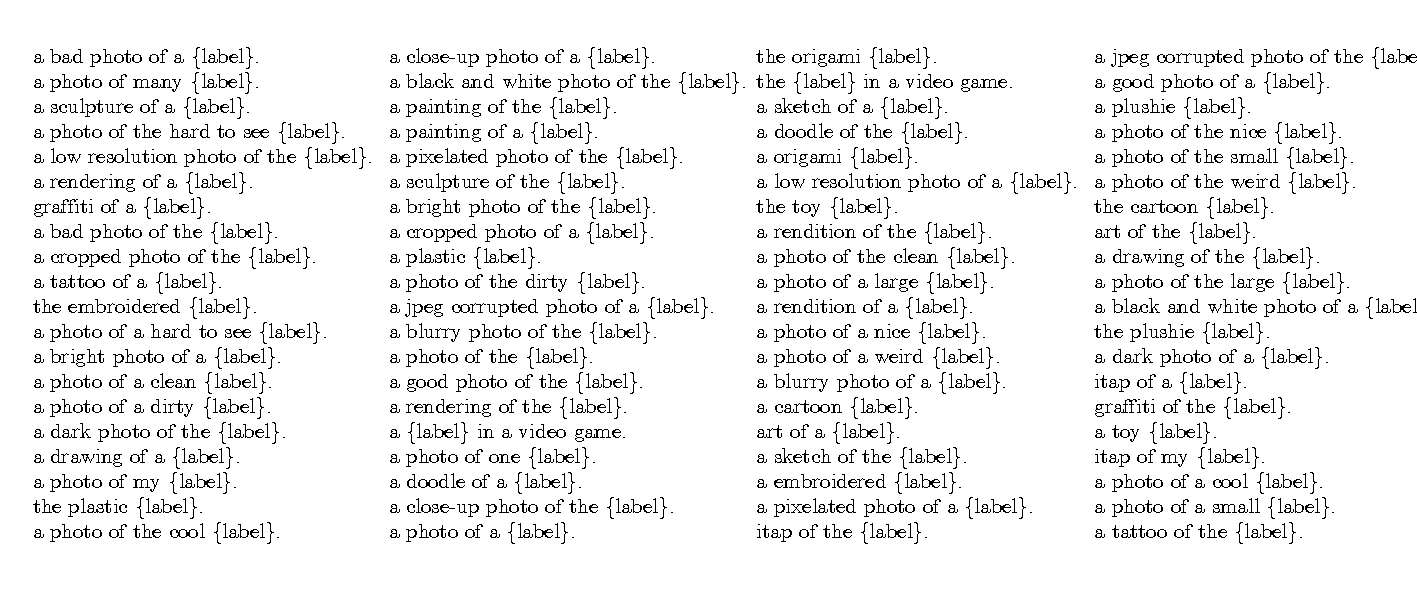
\includegraphics[width=1.0\columnwidth]{DeCLIP/figs/Prompts.pdf}
    \vskip -0.2in
	\caption{ The prompts for zero-shot testing. }
	\label{fig:prompts}
\end{figure}
% and the usage of prompts such as  \texttt{"a photo of a \{label\}"} improves the accuracy for classification tasks.

% The context information corresponding to each category uses prompts to make up, such as \texttt{"a photo of a \{label\}"}, and for the context of each category, we merged 80 prompts to generate.


\section{Additional study}\label{Additional study}

\begin{table*}[h]
% \vspace{3em}
\caption{\label{tab:ablation on datasets} \workname zero-shot performance of ImageNet top1 on different training datasets.}
\label{sample-table}
\begin{center}
\begin{footnotesize}
\begin{sc}
\begin{tabular}{ccccc}
  \toprule  
  %\multicolumn{5}{r}{}  \\
  \textbf{Backbone} & \textbf{Dataset}   & \textbf{Data Size}   &\textbf{Batch Size}  & \textbf{Zero-shot} \\
  \midrule   
  ResNet50 &ConceptualCaptions &3M  & 2,048 &27.8 	\\
  ResNet50 &Conceptual12M      &11M  & 4,096 &41.0 	\\
  ResNet50 &YFCC               &15M  & 4,096 &41.9 	\\
  \midrule   

  ResNet50 &DeCLIP open-source data &29M  & 6,144 &49.3 	\\
  \bottomrule
\end{tabular}
\end{sc}
\end{footnotesize}
\end{center}
% \vspace{-1.2em}
\end{table*}


\paragraph{Different Pre-training Datasets}
Data is critical for language-image pre-training task. 
% A large amount of data and extensive domain training pre-training models will bring better results to downstream tasks. 
As shown in Tab.~\ref{tab:ablation on datasets}, we evaluate our \workname on different sources of datasets.
% In Table \ref{tab:ablation on datasets}, we compare the training results of different source datasets. The last column is the evaluation results of ImageNet zero-shot top1 accuracy.
Combining Tab.\ref{tab:ablation on datasets} and Fig.\ref{fig:IN_zero_shot}, we can see that when the amount of training data continues to scale up, the zero-shot recognition ability continues to improve as well. In addition, we can see that the open source data has high quality. 
The 29M open source data can achieve 49.3\% zero-shot top1 accuracy on ImageNet through the \workname training paradigm.
% \workname combines open source data to create a dataset for academia and industry. 
Our open-source data is an affordable benchmark, which would be beneficial for explorations.
% This is a small but very effective benchmark, which allows to try explorations related to visual language pre-training with less computing resources.





\paragraph{Our YFCC re-implementation}

Although we use the same number of image-text pairs as the CLIP YFCC-15M, our YFCC data is different from CLIP. We also reproduce the naive CLIP on our YFCC-15M data, which results in 35.9\% zero-shot top1 accuracy on ImageNet-1K (see Fig.~\ref{tab:ablation on YFCC}). It is relatively higher than the number in CLIP paper (31.1\%). We conjecture the improvements might be caused by the different data cleaning strategies. However, our \workname can achieve 41.9\% zero-shot accuracy which is also 6.0\% higher than our CLIP re-implementation.

% We also train full setups of \workname on the YFCC15M dataset to compare the results of CLIP. Tabel \ref{tab:ablation on YFCC} is the comparison result of our approach and CLIP zero-shot top1 accuracy on ImageNet, using the same encoder and training data size. We can see that the 41.9\% zero-shot of \workname compare to zero-shot 35.9\% of reproduced CLIP, which is an amazing 6.0\% improvement on the YFCC15M dataset. In addition, we use the linear probe method to evaluate the pre-training model, which is trained on YFCC15M dataset, on the Fowers, Stanford Cars and ImageNet datasets. It can be seen from Table \ref{tab:YFCC downstream result} that our approach has 2.0\% improvement on the Fowers, 5.5\% improvement on the Stanford Cars, and 5.5\% improvement on the ImageNet. It is worth noting that the zero-shot we reproduced is higher than the report of CLIP, but the linear probe is lower than the report. This may be due to YFCC15M dataset differences. In addition, we use more stringent text cleaning rules to get high quality text, this will improve the zero shot ability, but may not improve the pre-training ability. Overall, \workname exceeds reported CLIP both zero-shot result and linear probe result on the YFCC15M dataset. This result further proves the strong generalization ability of our paradigm.






\begin{table*}[h]
\caption{\label{tab:ablation on YFCC} \workname zero-shot performance of ImageNet top1 on YFCC datasets. Although we use the same amount of data, our YFCC is different with CLIP YFCC due to the different data cleaning strategies.}
\begin{center}
\begin{small}
\begin{sc}
\begin{tabular}{cccccc}
  \toprule  
  %\multicolumn{5}{r}{}  \\
  \textbf{Model} &\textbf{Backbone} & \textbf{Dataset}   & \textbf{Data Size}   &\textbf{Batch Size}  & \textbf{Zero-Shot} \\
  \midrule   
  CLIP &ResNet50 &YFCC               &15M  & — &31.3 	\\
  CLIP (our reimp.) & ResNet50 &YFCC*    &15M  & 4,096 &35.9 \\
  \textbf{DeCLIP} &\textbf{ResNet50} &\textbf{YFCC*} &\textbf{15M}  &\textbf{4,096} &\textbf{41.9($\uparrow$+6.0)} 	\\
  \bottomrule
\end{tabular}
\end{sc}
\end{small}
\end{center}
\end{table*}


\paragraph{Memory usage}
Because of the additional views, our DeCLIP is more memory-consuming.
Thanks to the ICLR anonymous review comments: a fairer comparison might be doubling the batch size of CLIP.
Flowing the ablation study in Fig.~\ref{fig:abl_training_time}, we double the batch size and train CLIP-ResNet50 for 64 epochs. The final result is 22.3\% which is still 4.9\% lower than our DeCLIP model. We summarize the memory usage, training cost, and the final accuracy as below. All experiments are conducted on CC-3M with 16 V100 GPUs.

\begin{table*}[h]
\caption{\label{tab:ablation on memory usage} Ablation on Memory usage.}
\begin{center}
\begin{scriptsize}
\begin{sc}
\begin{tabular}{cccccc}
\toprule
\textbf{Model}           & \textbf{batch size per GPU} & \textbf{Memory (GB)} & \textbf{Epochs} & \textbf{Cost (GPU hours)} & \textbf{Zero-shot} \\
\midrule
CLIP-ResNet50   & 128                 & 15.8              & 64     & 416                       & 21.7                       \\
CLIP-ResNet50   & 256                 & 24.0              & 64     & 399                     & 22.3                        \\
DeCLIP-ResNet50 & 128                 & 22.7              & 32     & 304                       & 27.2 \\ 
\bottomrule
\end{tabular}
\end{sc}
\end{scriptsize}
\end{center}
\end{table*}